\documentclass[9pt,twocolumn,twoside,lineno]{pnas-new}
% Use the lineno option to display guide line numbers if required.

\templatetype{pnasresearcharticle} % Choose template 
% {pnasresearcharticle} = Template for a two-column research article
% {pnasmathematics} %= Template for a one-column mathematics article
% {pnasinvited} %= Template for a PNAS invited submission

\title{Learning Increases the Functional Connectivity Between Hippocampal CA1 neurons}

% Use letters for affiliations, numbers to show equal authorship (if applicable) and to indicate the corresponding author
\author[a,b,1]{Keiland W. Cooper}
%\author[b,1,2]{Author Two} 
%\author[a]{Author Three}

\affil[a]{Psychological and Brain Sciences, Indiana University Bloomington}
\affil[b]{Program in Cognitive Science, Indiana University Bloomington}

% Please give the surname of the lead author for the running footer
\leadauthor{Cooper} 

% Please add here a significance statement to explain the relevance of your work
\significancestatement{This research finds that the functional connectivity of the spiking hippocampal neurons networks increases its functional connectivity after learning, which adds support to previous whole brain findings using fMRI. The application of graph theoretics to neuronal hippocampal spiking data is also important to bridge scales across neuroscience disciplines. }

% Please include corresponding author, author contribution and author declaration information
\authorcontributions{Keiland Cooper wrote the network analysis and wrote the manuscript. GB collected the data.}
\authordeclaration{The author declares the only conflict of interest was that he would like a good grade on the final}
%\equalauthors{\textsuperscript{1}A.O.(Author One) and A.T. (Author Two) contributed equally to this work (remove if not applicable).}
\correspondingauthor{\textsuperscript{1}To whom correspondence should be addressed. E-mail: kc42\@iu.edu}

% Keywords are not mandatory, but authors are strongly encouraged to provide them. If provided, please include two to five keywords, separated by the pipe symbol, e.g:
\keywords{Hippocampus $|$ Networks $|$ Connections $|$  Final $|$  Project} 

\begin{abstract}
Learning and memory are key brain functions required for an uncountable number of cognitive and behavioral abilities, and understanding how they occur at the neural level is important for education, health, and even artificial intelligence research. A key brain region of the learning and memory system is the hippocampus, which is required for the formation and further recall of episodic memory. While it has received a considerable amount of attention, it is still unknown how learning effects the dynamics of populations of cells in the region. To address this deficit in knowledge of the hippocampus' functioning, spiking activity of 80+ cells was recorded in behaving rats before, during, and after spatial learning in behaving rats. Functional connectivity matrices were constructed using this data and further analyzed using graph theoretic approaches. General analysis of the network dynamics between the three phases revealed an increase in connectivity during and after learning had occurred. Community analysis corroborated these results, revealing that communities of nodes become less segmented after learning. Taken together, these findings add support to the theory that learning increases the homogeneity in brain networks, and may ultimately lead to a deeper understanding of how learning and memory are achieved by the brain.
\end{abstract}

\dates{This manuscript was compiled on \today}
\doi{\url{www.pnas.org/cgi/doi/10.1073/pnas.8675309}}

\begin{document}

\maketitle
\thispagestyle{firststyle}
\ifthenelse{\boolean{shortarticle}}{\ifthenelse{\boolean{singlecolumn}}{\abscontentformatted}{\abscontent}}{}

% If your first paragraph (i.e. with the \dropcap) contains a list environment (quote, quotation, theorem, definition, enumerate, itemize...), the line after the list may have some extra indentation. If this is the case, add \parshape=0 to the end of the list environment.
\dropcap{S}ince the early work of Brenda Milner and her amnesic patient HM \cite{scoville1957loss}, the medial temporal lobe brain regions have been the locus for understanding the neural correlates of how the brain learns and remembers. Over a decade later, we now know that the proper functioning of the region is required for memory formation and some forms of memory recall \cite{fyhn2007hippocampal}. This region, comprised of the entorhinal cortices, parahippocampal cortices, hippocampus, subiculum, and others \cite{scoville1957loss}, has been well studied over the last few decades. The hippocampus has particularly received a considerable amount of attention, due to the particular effects which have been reported given lesioning or physiological malformalities \cite{scoville1957loss}, \cite{grosmark2016diversity}. Numerous studies have discovered various properties of the hippocampus, such as place fields \cite{fyhn2007hippocampal}, which are studied cells that increase their firing rate in a given location, or oscillatory properties, such as theta and gamma oscillations. While a great deal of work has spanned both of these scales of hippocampal study, less is known about the interaction between multiple cells in the hippocampus.

First defined by Hebb, this complex network phenomena of neuronal assemblies have been defined as groups of neurons that are recruited together and activated concurrently, through synaptic connections between them, or functionally, given some stimulus \cite{pastalkova2008internally}. Neurons which display similar spiking patterns could be thought to be functionally connected, working together to represent a stimulus pattern in the environment, or a cognitive process within the brain. In some regards, these may be considered the smallest unit of neural representations in the brain and hippocampus. In the hippocampus, these groups of neurons could be considered the carriers of mnemonic information. For example, groups of place fields can be shown to represent an environment \cite{fyhn2007hippocampal}.

Moreover, these neuronal cellular assemblies are not static representations  \cite{pastalkova2008internally}. Instead, they dynamically alter over time. For hippocampal place cells, when an animal enters a new environment, the same group of neurons which represented the prior environment alter their firing rates accordingly, known as place field remapping. While other analysis have been used, graph theory provides the language and the tools \cite{rubinov2010complex} to parse these changes over a group of cells by analyzing the relationships between them. With this language, these learning induced alterations carried by the neurons could be considered a mechanisms of which the brain learns at the lowest level of representation, where the functional network of cell spiking dynamically changes to carry the new information. The properties of the network level functional connectivity of a population of neurons after learning however, is unknown.

To understand these properties further, a population of hippocampal CA1 neurons were recorded \cite{grosmark2016diversity} in four behaving rats over three phases: before learning during rest (PRE), during spatial learning (MAZE), and after learning during rest (POST). Similarity matrices were constructed from the neuron spiking data for each condition. Graph theoretic analysis were performed for each condition to track the changes before, during and after learning. The hypothesis was that learning will increase the connectivity of the network to account for the assimilation of new information and the formation of new connections between neurons. For ease of terminology, network will refer to neural networks in the biological sense, and graph will refer to the theoretical tools used to measure the association structure between neurons.



\section*{Results}
\subsection*{General Metrics}
For each phase in each rat, similarity matrices were computed by convolving the spike data with a gaussian kernel, and finding the correlations between each neurons convolved spike train. (Fig X). Nodes which did not show activity in a particular phase can be noticed from the long bands across the matricy. In addition, nodes which exhibited negative correlations were set to zero for ease of this analysis, and out of scope for this paper. Self connections, the long yellow band in the matricy, were not removed.

From the data, it is apparent that the networks become more correlated during the MAZE phase than the other two rest phases. Slightly more connectivity can be noticed in the POST phase matricy, as accounted for by the increase in the correlation coefficients closer to one. Thus, after learning the animal exhibited more connectivity in the network.


\begin{figure*}[tbhp]
\centering
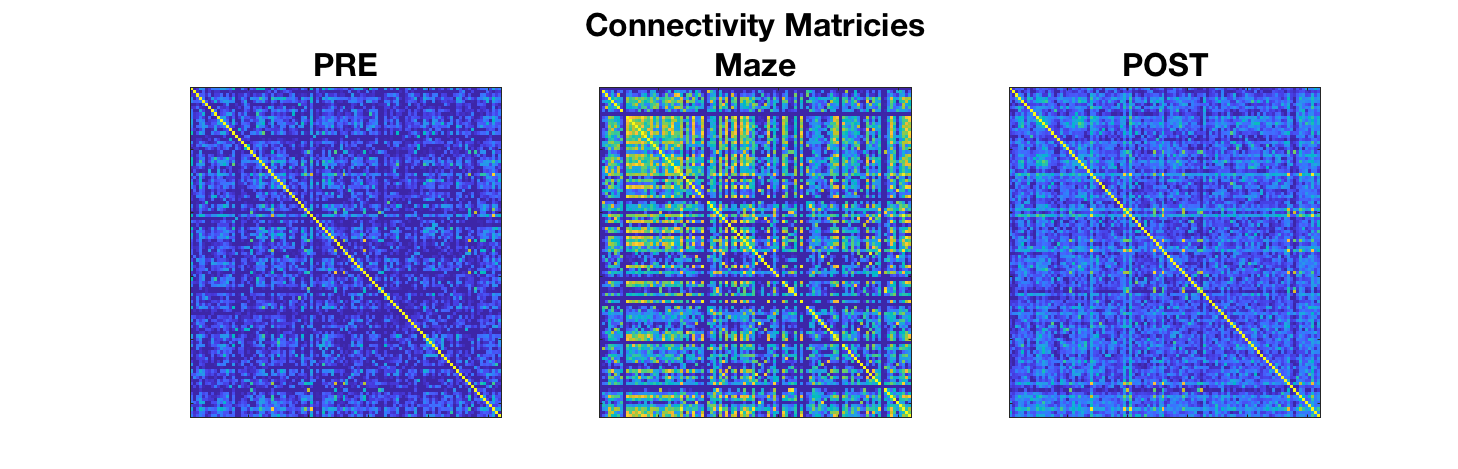
\includegraphics[width=.8\linewidth]{achCIJ}
\caption{Exemplar similarity matricies for each phase from one rat. Dark blue = 0; Yellow = 1}
\label{fig:achCIJ}
\end{figure*}

Standard graph theoretic measures were applied to the similarity matrices. An example from one rat is displayed in Table 1. The number of nodes corresponds to the number of recorded cells in the animal, and the number of edges corresponds to the number of functionally connected cells with a positive correlation. It can be seen from the table that after learning, the number of edges in the network increases, which is indicative of an increase in connectivity.  The average similarity for each matrix was also computed. A large increase can be detected between the PRE and MAZE phases, revealing that the similarity of the network spike train increased during learning. 



\begin{table}[tbhp]
\centering
\caption{Exemplar General Graph Theoretic Metrics}
\begin{tabular}{lcccc}
Phase & num nodes & num edges & density & avg similarity\\
\midrule
 PRE & 104& 7536 & 0.70351 & 0.11894\\
MAZE & 104& 7674 & 0.71639 & 0.28500\\
POST & 104 &  10300 & 0.96154& 0.20215\\
\bottomrule
\end{tabular}

\addtabletext{Metrics for one of the rats used in the analysis}
\end{table}


The degree distribution was also calculated for each phase for each animal (Fig 2). Many nodes appear to have a large amount of connections, as opposed to typical degree plots where there are a few nodes with many connections, hubs, and less with fewer. This may be due to the connectivity calculation, and an analysis that computes only the largest functional connectivity values may mitigate this.  

\begin{figure}[tbhp]
\centering
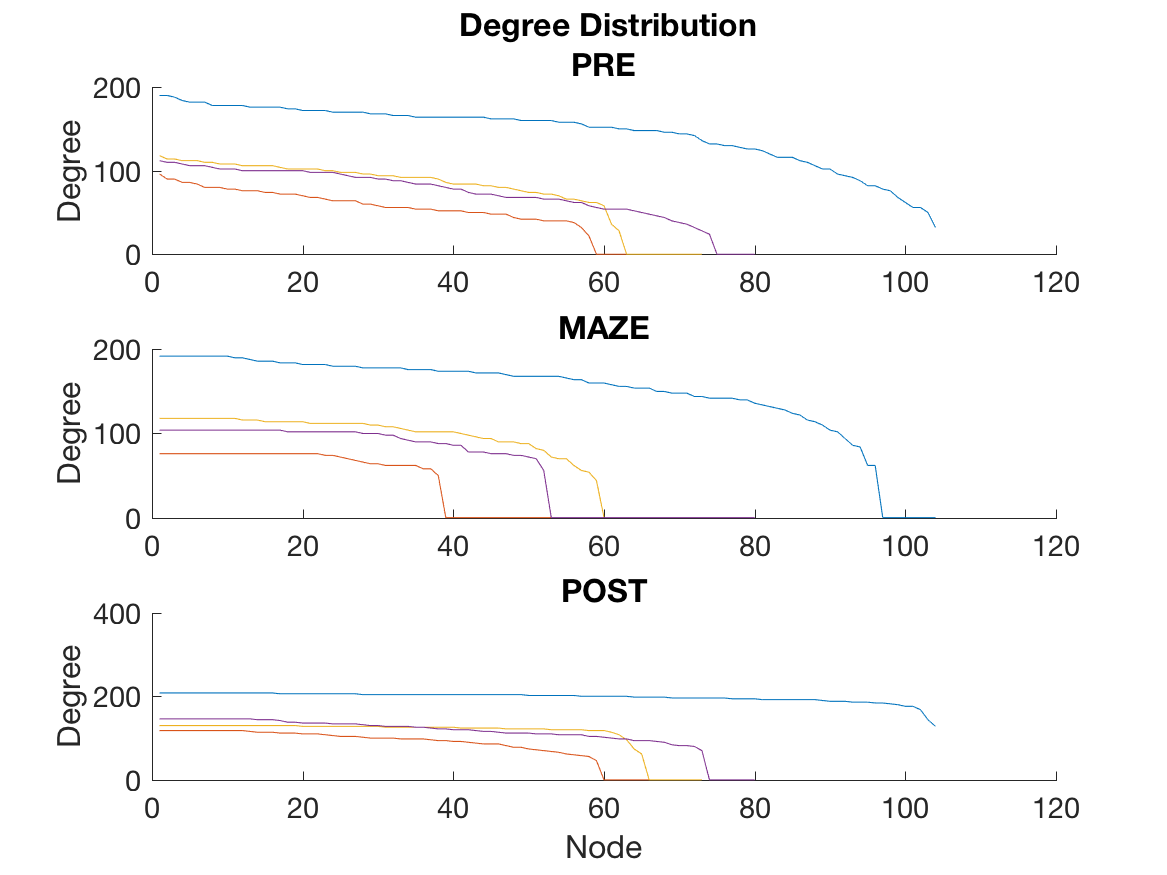
\includegraphics[width=.8\linewidth]{degs}
\caption{Degree distribution for each phase for each animal}
\label{fig:degs}
\end{figure}

The increase in node connectivity in the degree distribution was then further investigated. For each phase for each rat, the average degree was computed for each node (Fig 3). From the plot, the average degree decreases during the MAZE phase of the trial. This may be due to less nodes staying connected, or the presence of more hub like nodes. After this learning phase however, the average degree of the POST phase increases compared to the other two. This could be accounted for by the network becoming more connected after learning, and thus increases the average degree. This decrease and subsequent increase is consistent across the animals, and only slightly alters in slope between each of them.

\begin{figure}[tbhp]
\centering
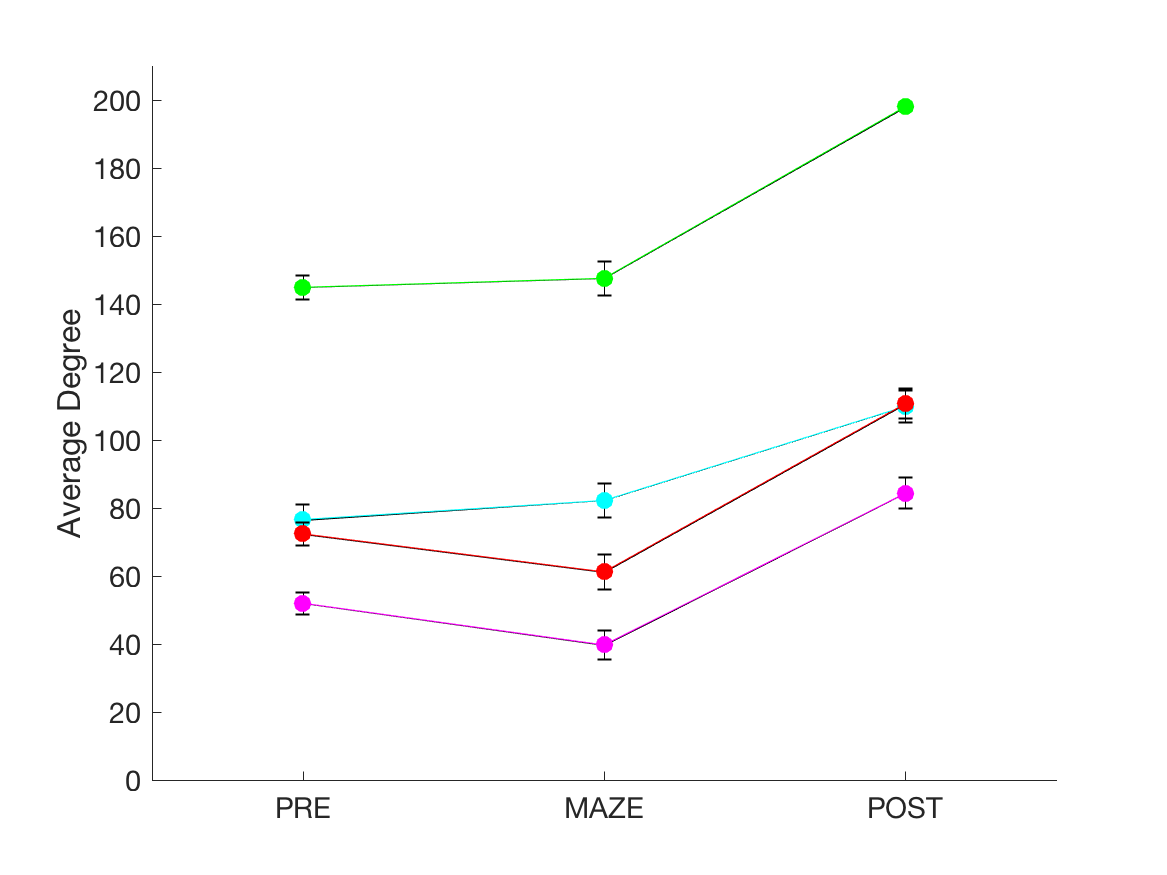
\includegraphics[width=.8\linewidth]{avgDeg}
\caption{Average Degree distribution for each phase for each animal}
\label{fig:avgDeg}
\end{figure}



\subsection*{Community Analysis}

Node communities, or nodes which form clusters with there edge connectivity, were then computed using 20 iterations of the Louvain community detection algorithm \cite{blondel2008fast}. The number of communities that were found by the algorithm were averaged over the iterations, and summarized in figure X. From this plot it can be seen that the average number of communities increases during the MAZE trial, sometimes quite sharply. After learning the number of communities again decreases, slightly lower than the original number. This could mean that nodes become more homogeneous, and are assimilated into other communities after learning occurs. This finding is consistent across rats, and the number of communities varies among them as well. Further analysis may parse whether this variance in number of communities can be accounted for by the different numbers of recorded neurons. Additionally, the sharp increases may be due to singleton nodes biasing the community calculation. Subsequent analysis will need to be performed to further parse this potential problem. It is unlikely that there are enough singletons to change this result, however. 


\begin{figure}[tbhp]
\centering
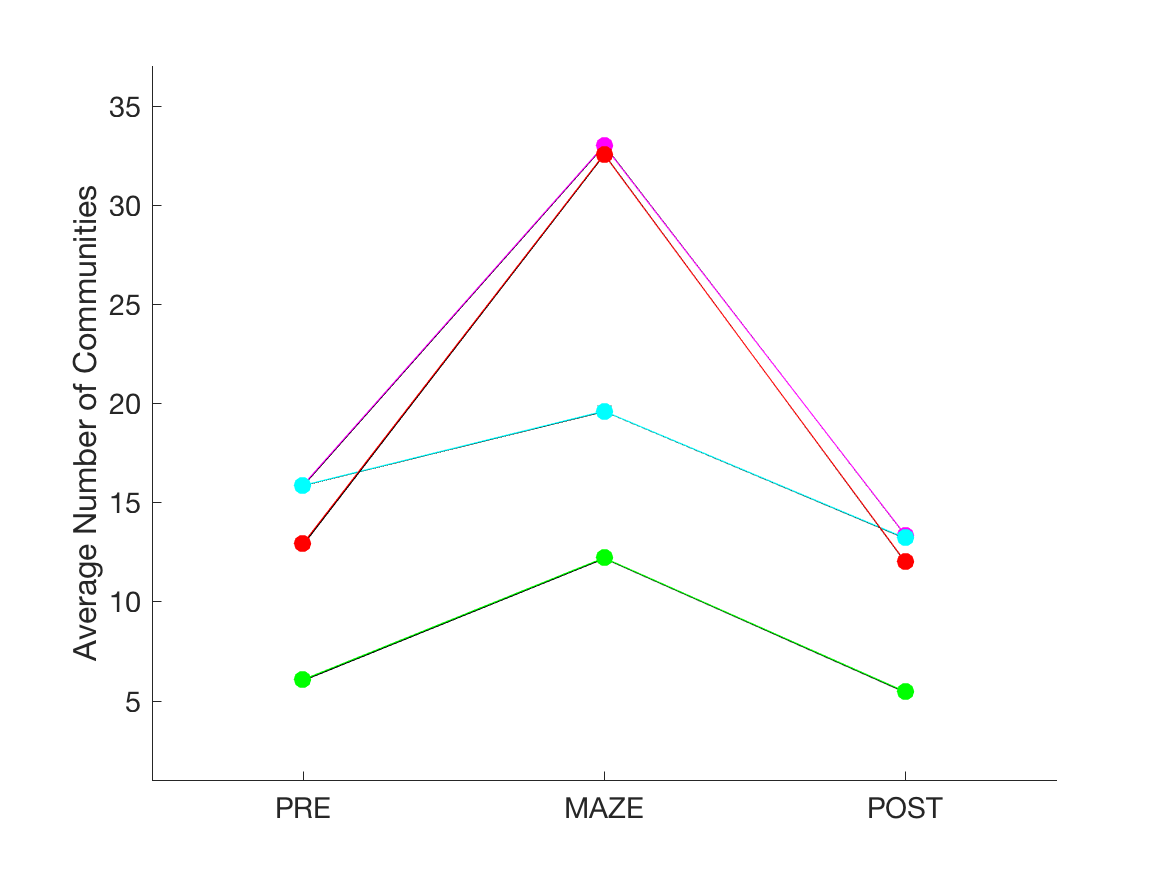
\includegraphics[width=.8\linewidth]{avgCi}
\caption{Average number of communities for each phase for each animal}
\label{fig:avgCi}
\end{figure}

Similarly, the average Q value was computed via the Louvain community detection algorithm (Fig 5). Q is a measure of modularity compartmentalization. Large Q values tend to be associated with many connections between the nodes within each community, but fewer connections to nodes outside of the community. Q was computed by taking the fraction of the edges that fall within the given communities found with the Louvain algorithm, minus the expected fraction if edges were distributed randomly in the graph. For this graph, the communities of the nodes during the earlier PRE phase are relatively compartmentalized. During learning in the MAZE phase, the communities decrease sharply in their Q values, and thus becoming more connected outside of their community assignments. after learning, in the POST phase, the lower Q values mean that the communities again become more segmented, but to a lesser degree than before the learning event. Ultimately, this may mean that learning increases the connectivity between the communities.


\begin{figure}[tbhp]
\centering
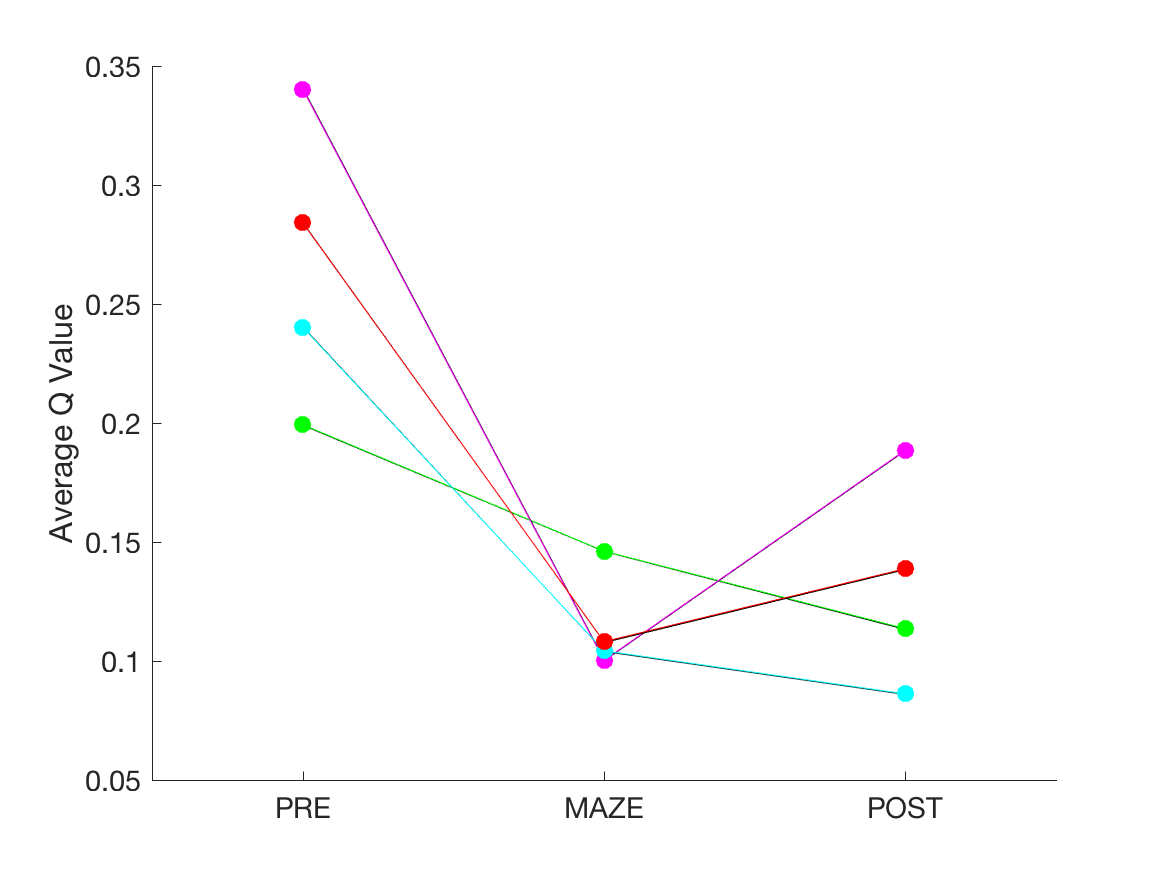
\includegraphics[width=.8\linewidth]{avgQ}
\caption{Average Q value for each phase for each animal}
\label{fig:avgQ}
\end{figure}


\section*{Discussion}
Hippocampal CA1 neurons were recorded in rats before, during, and after spatial learning  \cite{grosmark2016diversity}. Similarity matrices were constructed from the neuron spiking data for each of the three phases. Graph theoretic analysis \cite{rubinov2010complex} were performed for each condition to track the changes that occured between each phase.

To test the hypothesis that learning increases the functional connectivity between the population of neurons, both general and community analysis were computed. The general analysis revealed that the degree distribution of the networks dips during learning, and subsequently increases above the pre-learning baseline, after the learning has occured. Additionally, community analysis were performed to parse the changes between node connectivity over the phases. This analysis revealed that the communities were highly segmented before learning and then increased their connectivity outside of their community boundaries during learning. Post learning, the neurons again became more segmented in their community assignments, but ultimately became much more connected relative to the pre-learning baseline. Taken together, both of these analysis confirm the hypothesis that learning increases the connectivity of hippocampal neurons.

The dorsal region of hippocampal CA1 is largely associated with spatial learning and memory, largely due to the place cell studies which find the cells in the area. The spatial learning task that the animals performed would demonstrate new learning in this area, as the original report using this dataset had found \cite{grosmark2016diversity}. In this sense, learning would mean that the hippocampal neurons need to incorporate the new information from the novel environment into the current representations, or derive new ones to support further behaviors. It widely reported that during new learning, exploration, and movement, dorsal hippocampal cells exhibit rhythmic, 6-12 Hz synchronous activity known as theta, which has been hypothesised to drive connectivity in the region to aid LTP processes between neurons. This is confirmed by this analysis by the increase in correlation coefficients in the MAZE phase similarity matrices across animals. During rest and sleep, the oscillatory activity of the brain region decreases in frequency, with sparse synchronous activity, such as sharp waves or ripples. This decrease in overall synchronous activity is mirrored by the PRE and POST similarity matrices displaying lower correlation coefficients than during learning.

The similarity matrices were computed by convolving a gaussian kernel over the spiking data. This was due to the overt sparseness of the hippocampal spikes. This sparseness inherently introduces potential error in the correlation calculations, and in a handful of matrices a small percentage of neurons did not fire at all. This sparsity lowers the total number of neurons accounted for, and may bias the results that are reported. Further decreasing the number of neurons in the analysis, only neurons which exhibited positive correlations were analyzed. Further analysis may incorporate these neurons into the calculations, and could alter the results, though outside of the scope of this project.

The average increase in the degree distribution of the nodes in the graph may be inferred as neurons after learning becoming increasingly functionally connected across the network. This may be due to neurons forming new connections to support the learning, as well as to induce LTP processes within them \cite{pastalkova2008internally}. This increase in connectivity is in contrast to, during the learning phase, the average degree decreasing. This decrease during learning, taken together with the increase in correlation coefficients, may mean that the entire network is becoming synchronous with only a few of the neurons activities. If so, this would be an interesting area for further analysis to understand the dynamics of this "follow the leader" like phenomena. The degree distribution also stands out as odd, as it does not feature the typical power law found in many other brain networks. This may be a computational error, given the similarity matrices were not reduced by a threshold of neuron spike train correlations, to maintain the already low number of nodes in the analysis. It may additionally be a function of sampling bias in the dataset. Further exploration of possible reasons for the shape of this graph are required, however, if true, then this would mean that the hippocampal network does not form a few "hub" nodes, but rather many.

The community analysis revealed that the number of communities increased during learning. In terms of hippocampal dynamics, this could be due to segmenting existing neuronal assemblies to assimilate new learning. The subsequent increase in new communities forming could be from various input streams to the hippocampus coming online. The decrease in communities after learning may serve a consolidatory effect, whereby these new connections further segment into their respective communities. The increase in Q value after learning demonstrates this as well, and further reveals that these post-learning communities are more connected than they were before learning has occurred \cite{blondel2008fast}. Should this be the case, this new connectivity from the community structure may be the fingerprint of the learning process. Further studies may be done to parse if the communities found in the graphs have functional significance to the animal. For example, if one community of neurons represents a particular location in the maze, or some other qualitative feature. The reliability of this finding across animals may hint at a general property of hippocampal cell assemblies, where by the communities decompose and recompose continuously over time. Additional studies may be conducted that observes the temporal dynamics of this community composition after learning. The strong segmentation at baseline leads one to believe that the communities further segment after learning occurs. The precise dynamics associated with this may aid in understanding memory consolidation over time.


\matmethods{ 
All data and code used in this analysis can be found at \href{https://github.com/kwcooper/learningModsAssemblyNets}{github.com/kwcooper}.  

\subsection*{Data Collection}
Data was previously collected and explained in detail in (3). Briefly, simultaneous multi-cellular electrophysiological recordings of well-isolated CA1 pyramidal single units were performed in four Long-Evans rats. Eight bilateral silicon-probes were implanted into dorsal hippocampus of each rat. Each session consisted of three phases: a long (4 hour)  PRE rest/sleep epoch home-cage recordings performed in a familiar room, followed by a Novel MAZE running epoch (45 minutes) in which the naiive animals were transferred to a novel room, and water-rewarded to run on a novel maze. These mazes were either A) a wooden 1.6m linear platform, B) a wooden 1m diameter circular platform or C) a 2m metal linear platform. To encourage task participation, animals were given a reward at either at both ends of the linear platform, or at a predetermined location on the circular platform. The animal was gently encouraged to run unidirectionally on the circular platform. After the MAZE epochs the animals were transferred back to their home-cage in the familiar room where a long (4 hour) POST rest/sleep was recorded. Wide-band recordings were performed at 20 kHZ, and downsampled to 1250 HZ. Spike extraction and clustering was performed on the wideband (20 kHZ) signal and spike sorting was performed within a given silicon probe shank. 
\subsection*{Network Construction}
Spiking similarity networks were constructed for each of the three phases for each animal. Spikes times subsequently were sorted by neuron. Similarity between spike trains was computed by three methods, the Victor and Purpura method, the Van Rossum method, and by kernel convolved spike train correlations. Due to given constraints, only the latter method was subsequently used in the analysis. With this method, to overcome the sparsity in neural firing, spike trains were convolved with a gaussian kernel of size k, with $ \sigma  = \frac{k}{4} $ and $ c = \frac{k}{2} $. Similarity matrices were produced by computing the pairwise linear correlation coefficient between each pair of the convolved spike trains. Negative correlations and non-number values were removed for further analysis for graph theoretic computations.
\subsection*{Network Analysis}
For each phase for each rat, graph theoretic computations were performed using the Brain Connectivity Toolbox. Graph density, number of nodes, number of edges, and node degrees were computed with in-built functions. Characteristic path length, the average shortest path length between all pairs of nodes, and efficiency were computed using the weighted distance of the reciprocal of the similarity matrix. Optimal graph community structure, which segments the graph according to the minimization of edges between groups and maximization of edges within groups, was computed using a multi-iterative generalization of the Louvain community detection algorithm \cite{blondel2008fast}, over 20 iterations. Communities were ordered using a consensus clustering algorithm and an co-assignment matrix for plotting. 

}
\showmatmethods{} % Display the Materials and Methods section

\acknow{The author thanks Dr. Richard Betzel for fruitful discussions, guidance, and an all around amazing course.}

\showacknow{} % Display the acknowledgments section

% Bibliography
\bibliography{pnas-sample}

\end{document}